\Needspace{10\baselineskip}
\section{自研 RISC-V 处理器核}
\label{sec:core}
处理器核为自研 RV32IM 实现，v0 两级流水基线，v1 升级为三级流水并加入转发与分支预测。
微架构见图~\ref{fig:core}。
接口契约以 \code{design_v0.md} 与 \code{design_v1.md} 冻结版本为准。

\begin{figure}[H]\centering
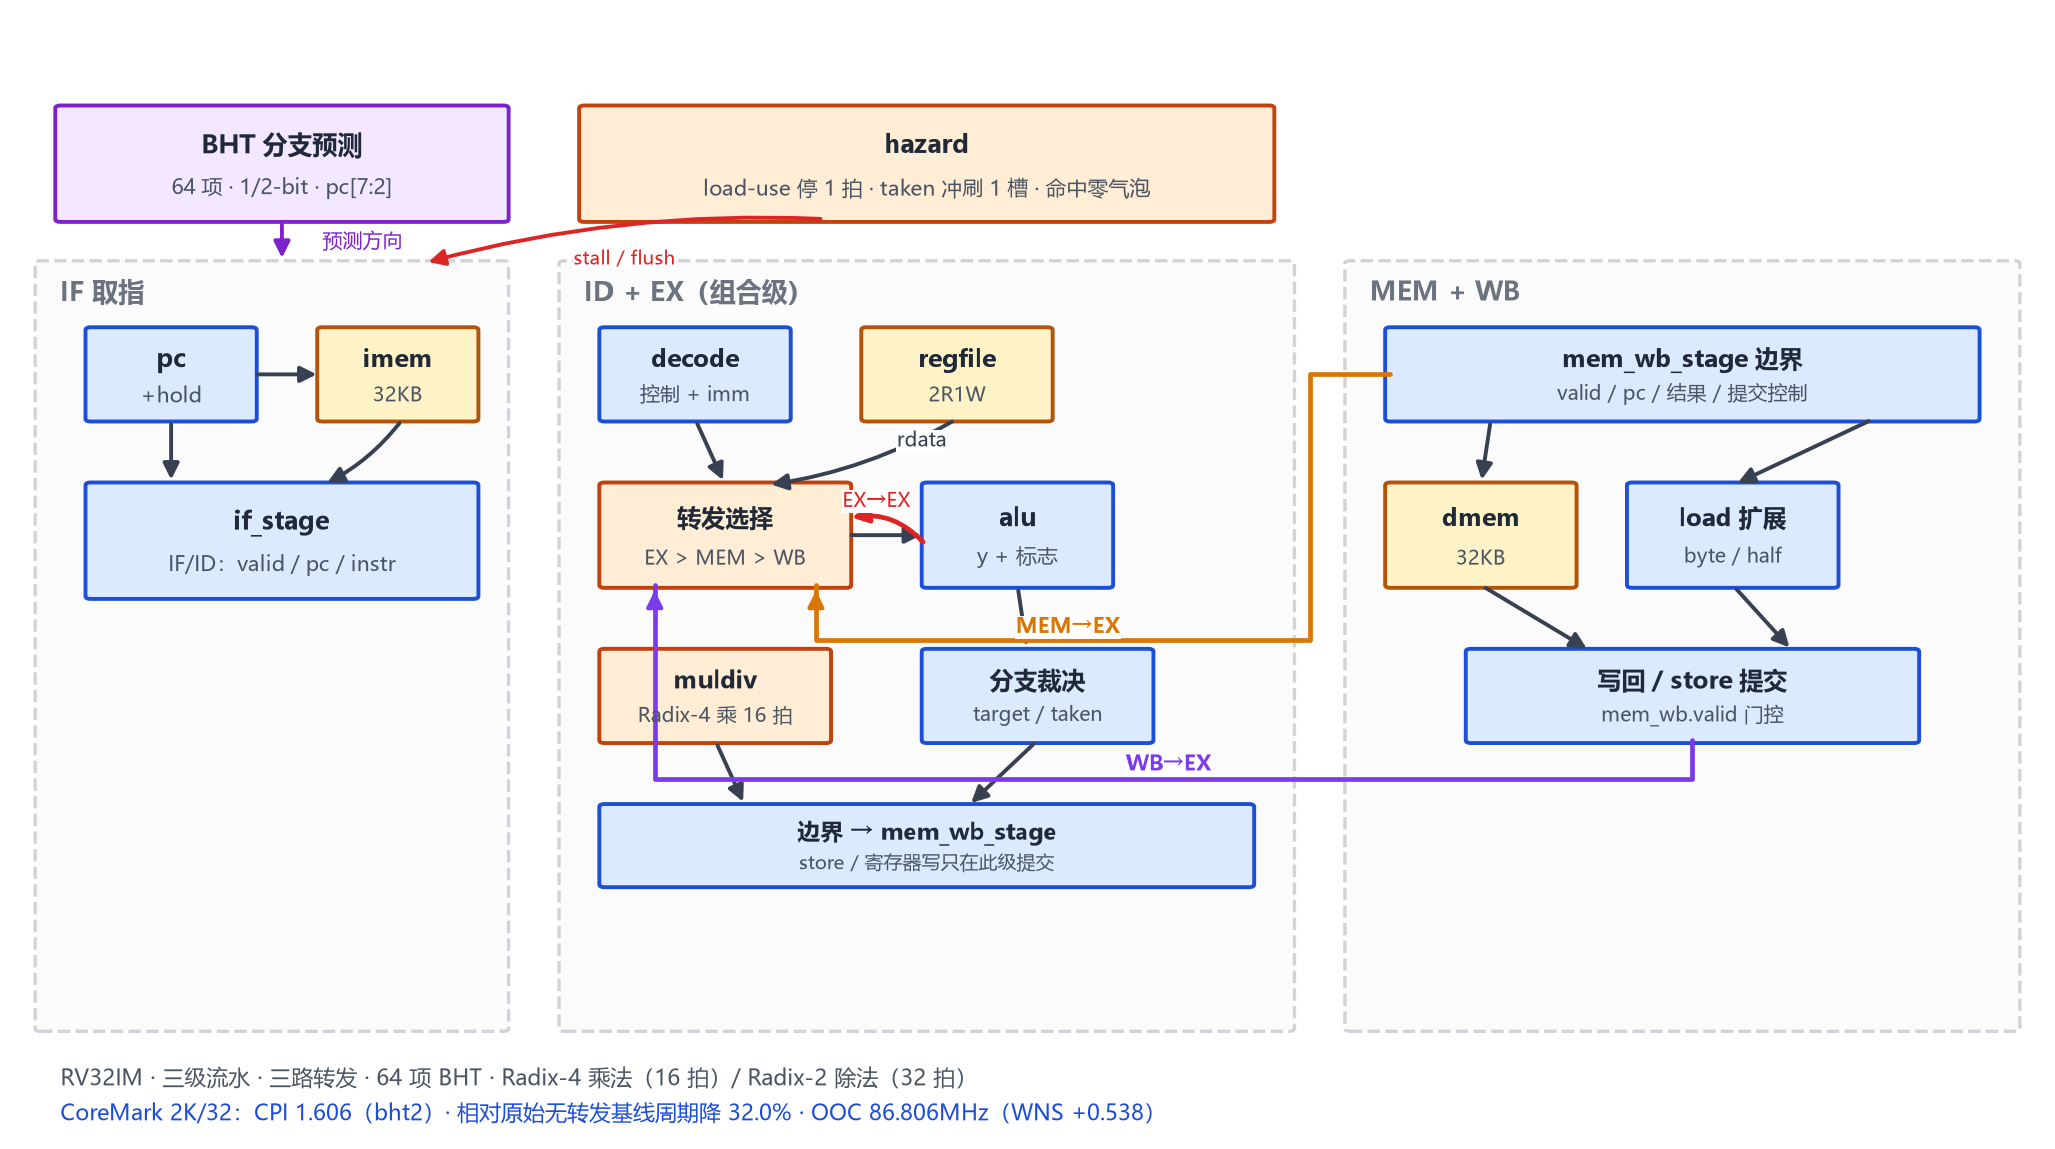
\includegraphics[width=0.98\linewidth]{fig_core.png}
\caption{RISC-V 三级流水、三路转发与 BHT（仓库配图）}\label{fig:core}
\end{figure}

\subsection{微架构}
v1 核为三级流水（IF/ID、EX/MEM、MEM/WB），三路转发优先级为 EX、MEM、WB、寄存器堆。
乘除法采用 Radix-4 基四乘法（16 次迭代）与 32 拍恢复除法，除零与 \code{INT_MIN/-1} 边界显式处理。
分支预测为 64 项 BHT，支持 1-bit 与 2-bit 两档，可经参数切换。
对照档为同一份 RTL 的参数开关，不维护第二份代码。

\subsection{性能：CoreMark 与分类记账}
CoreMark 统一 2K/32 iterations、-O2、统一退休口径；结果为仿真外推值，非官方认证分数。
四档数据见表~\ref{tab:coremark}。

\begin{table}[H]\centering\small
\caption{CoreMark 四档（retired 10{,}106{,}386 条指令）}\label{tab:coremark}
\begin{tabularx}{\linewidth}{@{}P{42mm}P{30mm}Y@{}}\toprule
配置 & CPI & CoreMark/MHz\\\midrule
v0 两级（外部锚点） & 2.105 & 1.506\\
v1 三级，无转发 & 1.886 & 1.681\\
v1 三级，转发 & 1.693 & 1.872\\
v1 三级，转发+BHT1 & 1.616 & 1.961\\
v1 三级，转发+BHT2 & 1.606 & 1.974\\\bottomrule
\end{tabularx}\end{table}

性能收益按优化项分类记账，不混记：固定 Radix-4 乘法器后开关转发，CPI 降幅 10.20\%；固定转发后更换乘法器，周期降幅 21.95\%；两项相对原始无转发基线的组合降幅 28.30\%；转发基础上启用 BHT2 再降 5.15\%。
25\% 为组合优化的尽力目标，未作为单一手段的门禁；原始 FAIL 数据永久保留。

\subsection{功能验证}
riscv-arch-test 以官方 golden 签名为判据：I+M 子集 44/44 签名匹配，档间签名一致。
官方 \code{beq-01} 用例超出 32 KB 链接上限（溢出 195{,}388 字节），故采用 3I+8M 子集，失败留证。
CoreMark 结果与宿主机 -O2、-O0 双档交叉核对，CRC 三方一致。
回归入口为 \code{sim/scripts/run_iverilog.sh}，tb 全部位于仓库内。

\subsection{时序与上板}
时序采用外推、实点、板上三档口径：\code{@10 ns} 约束下仅无转发档通过（WNS +0.051 ns）；BHT2 以 11.52 ns 独立约束实点通过，WNS +0.538 ns，对应 86.806 MHz（表~\ref{tab:coretiming}）。

\begin{table}[H]\centering\small
\caption{核 OOC 时序口径（WNS，ns）}\label{tab:coretiming}
\begin{tabularx}{\linewidth}{@{}P{46mm}P{26mm}Y@{}}\toprule
配置与约束 & WNS & 结论\\\midrule
v1 无转发 @ 10 ns & +0.051 & 通过\\
v1 转发 @ 10 ns & $-0.587$ & 未通过，留档\\
v1 转发+BHT1 @ 10 ns & $-0.419$ & 未通过，留档\\
v1 转发+BHT2 @ 10 ns & $-0.586$ & 未通过，留档\\
v1 转发+BHT2 @ 11.52 ns & +0.538 & 通过，实点 86.806 MHz\\\bottomrule
\end{tabularx}\end{table}

最小 SoC（核 + 32 KB 哈佛存储 + LED 外设）以 40 MHz 上板，WNS +3.618 ns，LUT 6{,}768、FF 859、BRAM 8、DSP 0，LED 显示与固件预期一致。
SoC 125 MHz 构建 WNS $-8.044$ ns，FAIL 记录保留，不作为当前能力声明。
\FloatBarrier
